\documentclass[a4paper,12pt]{article}
\usepackage[a4paper]{geometry}
\usepackage{color, hyperref}
\usepackage[hypcap]{caption}
\usepackage[utf8]{inputenc}
\usepackage{float}
\usepackage{array}
\usepackage{ulem}
\usepackage{contour}
\usepackage{listings}
\usepackage{booktabs}
\usepackage{multirow}
\usepackage{wrapfig, graphicx}
\usepackage{caption}
\usepackage{subcaption}
\usepackage{mathpazo}
\usepackage{sectsty}
% \allsectionsfont{\sffamily}
\usepackage[english]{babel}
\usepackage[T1]{fontenc}
\usepackage{fancyhdr}
\usepackage{xcolor} % où xcolor selon l'installation
\definecolor{Valentia}{RGB}{233,78,82}
\definecolor{Titleblue}{RGB}{114, 146, 162}
\usepackage{scrextend} % Forcer la 4eme  de couverture en page pair
\usepackage{multirow} %% Pour mettre un texte sur plusieurs rangées
\usepackage{multicol} %% Pour mettre un texte sur plusieurs colonnes
\usepackage[absolute]{textpos} 
\usepackage{titlesec}
\usepackage{tikz}
\usepackage{multicolrule}

\graphicspath{{./img}}

\definecolor{codegreen}{rgb}{0,0.6,0}
\definecolor{codegray}{rgb}{0.5,0.5,0.5}
\definecolor{codepurple}{rgb}{0.58,0,0.82}
\definecolor{backcolour}{rgb}{0.9,0.9,0.9}
\lstdefinestyle{myStyle}{
	backgroundcolor=\color{backcolour},
	commentstyle=\color{codegreen},
	keywordstyle=\color{magenta},
	numberstyle=\tiny\color{codegray},
	stringstyle=\color{codepurple},
	basicstyle=\ttfamily\footnotesize,
	breakatwhitespace=false,
	breaklines=true,
	captionpos=b,
	keepspaces=true,
	showspaces=false,
	showstringspaces=false,
	showtabs=false,
	tabsize=2,
	linewidth=\linewidth,
	xleftmargin=0.2\linewidth,
	% padding=5px
}

\lstset{style=myStyle}


\renewcommand{\ULdepth}{1.8pt}
\contourlength{0.8pt}

\newcommand{\ul}[1]{%
	\uline{\phantom{#1}}%
	\llap{\contour{white}{#1}}%
}

\captionsetup{labelfont={it, bf}, textfont={it}}

\pagestyle{fancy}
\fancyhf{}
\fancyheadoffset{0.005\textwidth}
\lhead{PolyMessages}
\rhead{Rapport Final}
\lfoot{Marvin B. | Eri A. | Lucas N.}
\rfoot{Page \thepage\ / 6}

\definecolor{black}{rgb}{0,0,0}
\definecolor{green}{rgb}{0,0.5,0}
\definecolor{red}{rgb}{1,0,0}
\definecolor{blue}{rgb}{0,0,1}
\hypersetup{
	colorlinks=true,
	breaklinks=true,
	linkcolor=black,
	urlcolor=cyan,
	pdftitle={PolyMessages - Sprint 3}
}

\renewcommand{\footrulewidth}{1pt}
%%%%%%%%%%%%%%%%%%%%%%%%%%%%%%%%%%%%%%%%%%%%%%%%%%%%%%%%%%%%%%%

% \titleformat{\section}
% {\titlerule
% \vspace{.8ex}%
% \Large\bfseries}
% {\thesection.}{.5em}{}

\titleformat{\part}[display]
{\bfseries\Large}
{\filleft PARTIE \Huge\thepart}
{0ex}
{\titlerule
\vspace{1ex}%
\filright}
[\vspace{1ex}%
\titlerule]

\captionsetup{labelfont={it, bf}, textfont={it}}
\setlength{\headheight}{15pt}
% \addtolength{\topmargin}{-2.5pt}

\begin{document}

\begin{titlepage}

\newgeometry{left=2.5cm, bottom=3cm, top=2cm, right=2.5cm}

\tikz[remember picture,overlay] \node[opacity=1,inner sep=0pt] at (73.6mm, -124.25mm){
\includegraphics{Fond.pdf}};

{\fontfamily{phv}\fontseries{mc}\selectfont
%*****************************************************
%******************** TITRE **************************
%*****************************************************
\centering
\color{Valentia}
\fontsize{18}{13}\selectfont
\textbf{Rapport de Projet Final}

\normalsize
\color{black}

\bigskip
\textbf{Informatique et Gestion}

\bigskip
\textbf{Polytech Montpellier}

\bigskip

\color{Titleblue}
\fontsize{17}{20.4}\selectfont
\vspace{2cm}
\textbf{POLYMESSAGES}

%*****************************************************

\vspace{4cm}
\fontsize{15}{18}\selectfont
\color{black}
\textbf{Présenté par Marvin BONTEMPS, Eri AGNESE et Lucas NOUGUIER\\
le 01 Juin 2022}

\bigskip
\fontsize{13}{15.6}\selectfont
\textbf{Sous la direction de Thomas GODEL}

\vspace{1.5cm}
\normalsize
\textbf{Devant le jury composé de}\\
\bigskip
\fontsize{10}{12}\selectfont
\vspace{1.5mm}
\begin{center}
	\textbf{Thomas GODEL}
\end{center}

%************************************
%**  LOGO  UNIVERSITÉ
%*****************************************************
\vspace{\fill}
\begin{center}
	
\includegraphics[height=60px]{LogoPolytech.png}
	\hfill
	
\includegraphics[height=65px]{LogoUM.png}
\end{center}
}
\end{titlepage}

%%%%%%%%%%%%%%%%%%%%%%%%%%%%%%%%%%%%%%%%%%%%%%%%%%%%%%%%%%%%%%
\newgeometry{top=2cm, bottom=2.5cm, left=2cm, right=2cm}

\tableofcontents
\clearpage
\hypersetup{linkcolor=red}

\section{Protocole de communication}
\begin{figure}[h]
	\centering
	\begin{subfigure}{0.45\linewidth}
		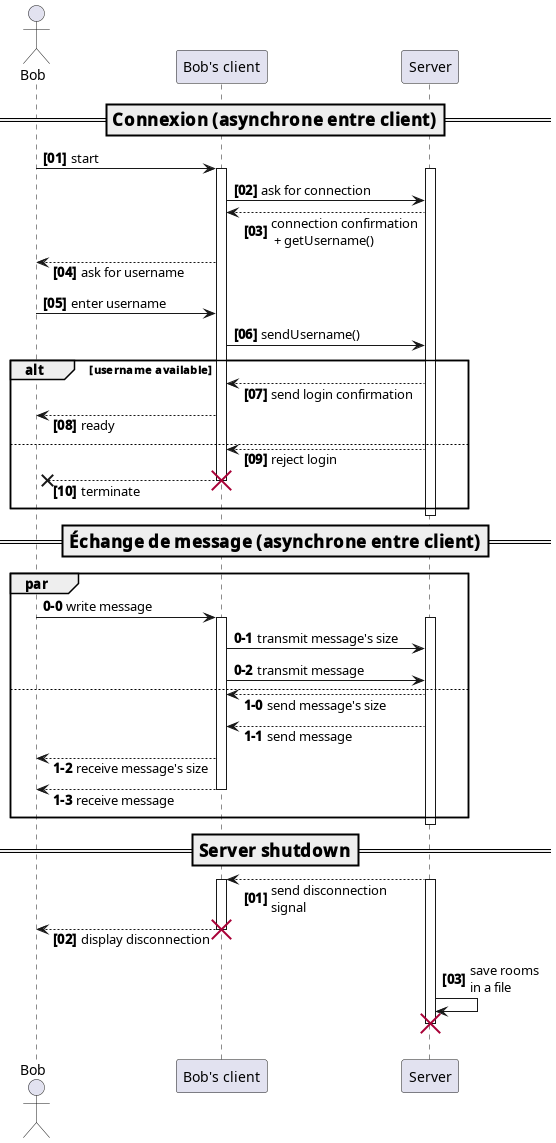
\includegraphics[width=\linewidth]{sequence.png}
		\caption{Fonctionnement global}
	\end{subfigure}
	\hfill
	\begin{subfigure}{0.45\linewidth}
		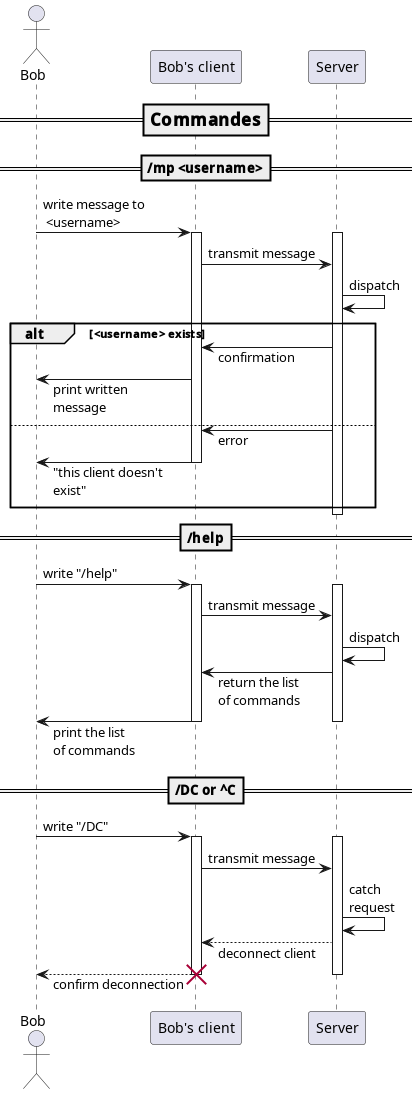
\includegraphics[width=0.8\linewidth]{commands.png}
		\caption{Protocole des commandes}
	\end{subfigure}
	\caption{Protocoles}
	\hrulefill
\end{figure}

\pagebreak

\begin{figure}[h!]
	\ContinuedFloat
	\centering
	\begin{subfigure}{0.45\linewidth}
		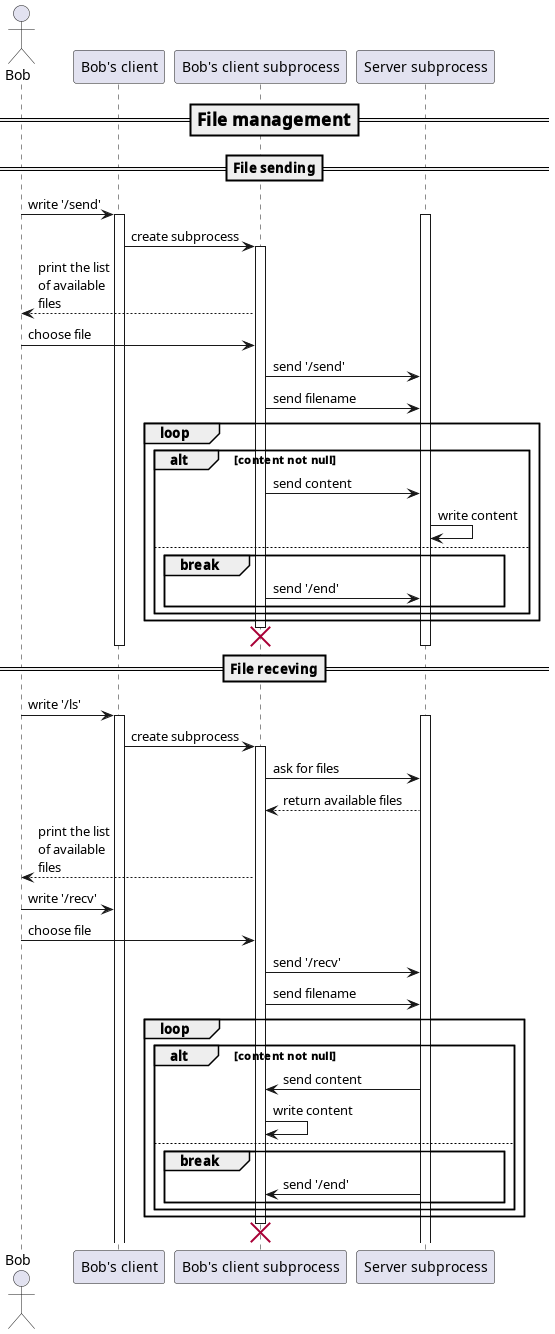
\includegraphics[width=\linewidth]{fileManagement.png}
		\caption{Protocole d'échange de fichiers}
	\end{subfigure}
	\hfill
	\begin{subfigure}{0.45\linewidth}
		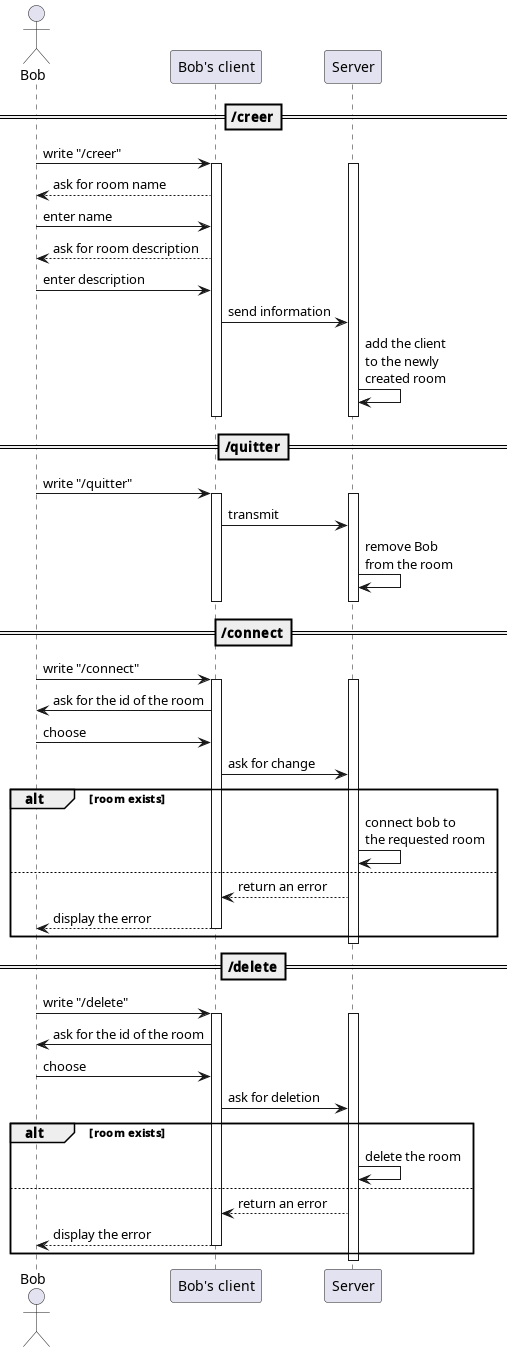
\includegraphics[width=0.9\linewidth]{rooms.png}
		\caption{Protocle des salons}
	\end{subfigure}
	\caption{Protocoles}
	\hrulefill
\end{figure}

\pagebreak
\section{Architecture}
\begin{figure}[h]
	\centering
	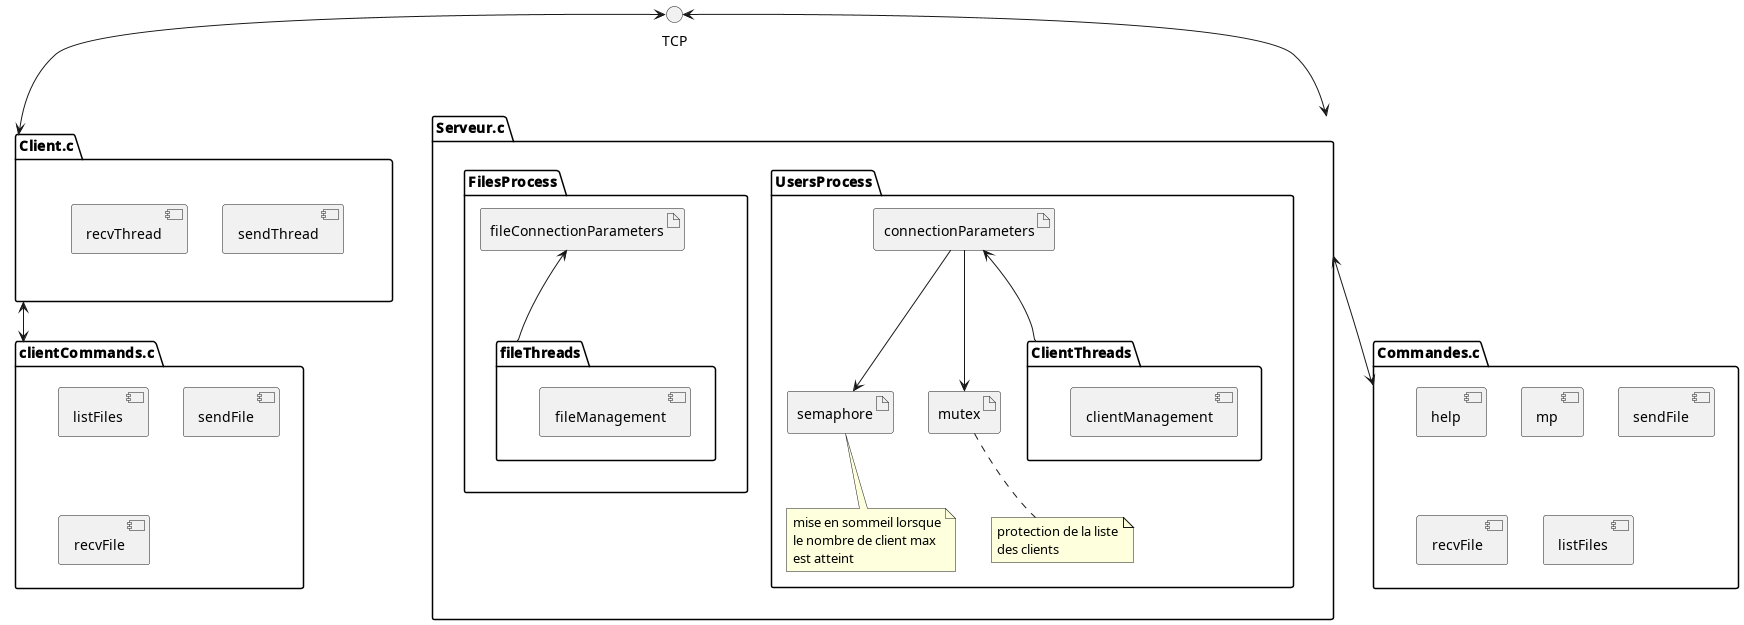
\includegraphics[width=\linewidth]{architecture.png}
	\caption{Architecture de la messagerie}
	\hrulefill
\end{figure}
\section{Répartition du travail}
\begin{wraptable}{r}{0.55\linewidth}
	\vspace{-0.5cm}
	\begin{tabular}{cccc}
		\toprule
		\multirow{2}{*}{Tâches} & \multicolumn{3}{c}{Étudiants}\\
		& Lucas & Éri & Marvin\\
		\midrule
		Finalisation fichiers & X\\
		\midrule
		Création des salons & & X & X\\
		\midrule
		Destruction des salons & & X &\\
		\midrule
		Connection aux salons & X\\
		\midrule
		Deconnection des salons & & X\\
		\midrule
		Rédaction du guide & & & X\\
		\bottomrule
	\end{tabular}
	\caption{Tâche effectuée par étudiant}
	\label{table:repartition}
\end{wraptable}
La 4\textsuperscript{ème} version de la messagerie consistait à rajouter en priorité une fonctionnalité de salons textuels permettants aux clients de discuter de manière plus privée ailleurs que sur le salon général. Pour cela, nous avons d'abord implémenté une commande permettant de créer des salons et de leur donner un nom et une description, ensuite nous avons codé la fonction permettant d'énumérer les différents salons présents sur le serveur ainsi que la fonctionnalité pour se connecter à un salon et celle permettant de s'en déconnecter. Pour finir, nous avons rajouté la fonction permettant la suppression d'un salon.

Nous n'avons malheureusement ni réussi à ajouter la possibilité de modifier les noms et descriptions des salons, ni réussi à implémenter la fonctionnalité permettant de restaurer les salons à l'allumage du serveur et nous n'avons pas eu le temps de rajouter des fonctionnalités supplémentaires.

\begin{figure}[h!]
	\centering
	\vspace{0.4cm}
	\begin{subfigure}{\linewidth}
		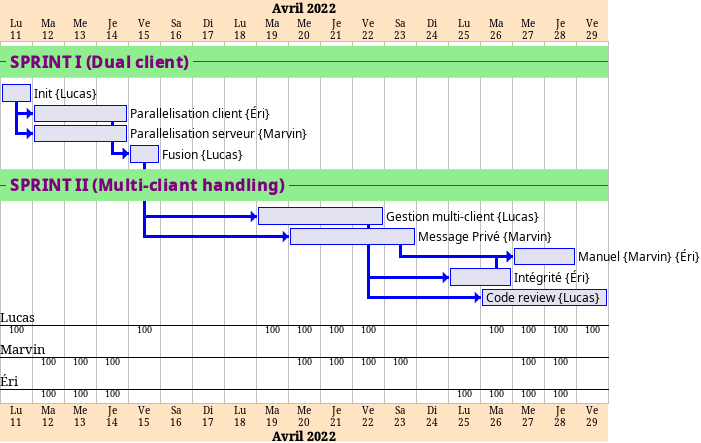
\includegraphics[width=\linewidth]{gantt.png}
		\caption{Sprint I \& II}
	\end{subfigure}
	\begin{subfigure}{\linewidth}
		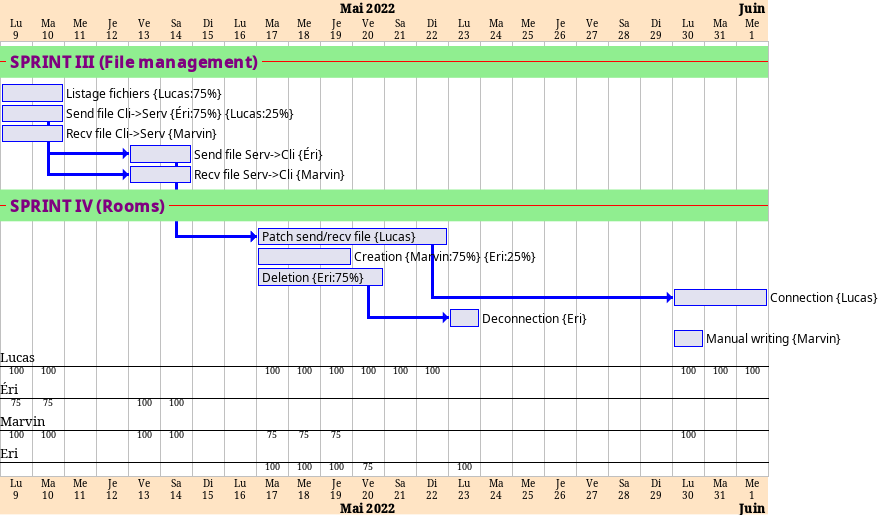
\includegraphics[width=\linewidth]{gantt2.png}
		\caption{Sprint III \& IV}
	\end{subfigure}
	\caption{Diagramme de Gantt sur la réalisation du projet}
	\label{fig:gantt}
	\hrulefill
\end{figure}
\pagebreak
\section{Exécution du code}
Pour lancer la messagerie, il faut commencer par compiler et lancer le serveur en spécifiant les 2 ports (1: port d'écoute pour les messages, 2: port d'écoute pour les fichiers)
\begin{figure}[h]
	\centering
	\vspace{-0.1cm}
	\begin{lstlisting}[language=bash, gobble=4]
		[lucas@xps-lucas ~]$ gcc -o server serveur.c commandes.c
		[lucas@xps-lucas ~]$ ./server <PORT1> <PORT2>
	\end{lstlisting}
\end{figure}

\noindent On peut alors lancer les clients en spécifiant les mêmes ports que pour le serveur
\begin{figure}[h]
	\centering
	\vspace{-0.2cm}
	\begin{lstlisting}[language=bash, gobble=4]
		[lucas@xps-lucas ~]$ gcc -o client client.c clientCommands.c
		[lucas@xps-lucas ~]$ ./client <IP> <PORT1> <PORT2>
	\end{lstlisting}
\end{figure}
\section{Difficultés}
\begin{itemize}
	\item Les fonctionnalités du sprint précédent n'étaient pas opérationnelles, il y a donc eu une prise de retard sur les fonctions à implémenter lors de ce sprint puisqu'il a fallu terminer les fonctions concernant l'envoi des fichiers
	\item A la fin, lors de la fusion des travaux, une erreur d'allocation mémoire s'est invitée dans la commande permettant de lister les salons et son origine n'a pas pu être trouvée.
	\item Pour la création des salons, nous avons eu au départ un problème car on ne pouvais pas mettre d'espace dans le nom ni dans la description du salon, on a finalement réglé ce problème en utilisant un fgets à la place d'un scanf
\end{itemize}
\end{document}